\documentclass[12pt,letter]{article}
\usepackage[moduleName={Pallet Town Waves System}]{KautenjaDSP}
% import a debugging package to show the margin boxes
% \usepackage{showframe}
% set the graphics path to the img directory
\graphicspath{{img/}}

% algorithm2e stuff
% \SetKwInOut{Objects}{$\CKmatrix{O}$}
% \SetKwInOut{Weights}{$\CKvector{w}$}

\begin{document}
\titlePage{Logo}{Module}{KautenjaDSP}

% -------------------
% MARK: Overview
% -------------------

\section*{Overview}

Pallet Town Waves System is an emulation of the Nintendo GameBoy Sound System (GBS) audio processing unit. The GBS contains two pulse wave generators, a wavetable oscillator, and a noise generator. Pallet Town Waves System provides the key features of the GameBoy Sound System chip, namely,
\begin{itemize}
  \item \textbf{Dual pulse wave generator:} Dual pulse waveform generator with duty cycles of $12.5\%$, $25\%$, $50\%$, and $75\%$; and 11-bit frequency value
  \item \textbf{Wave-table oscillator:} bank of 5 discrete 4-bit Waveforms with length of 32 samples that can be interpolated between smoothly
  \item \textbf{Noise generator:} generate pseudo-random numbers at 7 different frequencies
  \item \textbf{4-bit Amplifier:} A 4-bit amplifier controls the output level of each oscillator with base/attenuator knobs and CV inputs (with exception of the wave waveform, which has four volume levels)
  \item \textbf{Channel Mixer:} Mix the voices together internally with hard clipping and intentional aliasing
\end{itemize}

% -------------------
% MARK: Panel Layout
% -------------------

\clearpage
\section*{Panel Layout}

\begin{figure}[!htp]
\centering
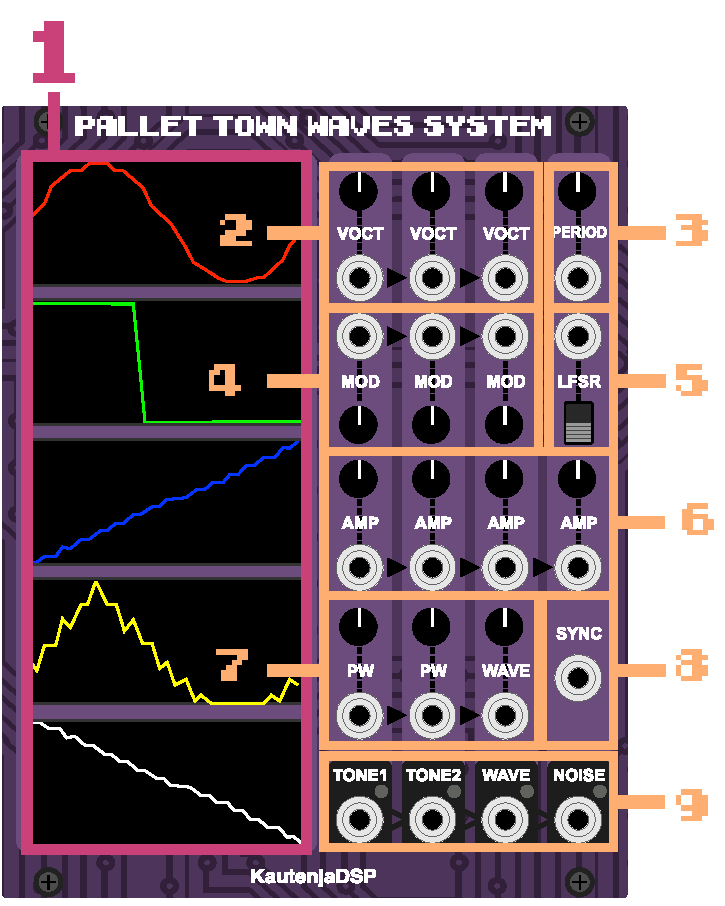
\includegraphics{Interface}
\end{figure}

\subsection*{1{\quad}Frequency}

The trimpot controls the coarse frequency of the three waveform generators. Frequency is quantized to a 11-bit value for the oscillators, which is particularly noticeable in the very low / high registers. The ports provide an exponential $V$/Octave input for controlling the pitch of the waveform generators. Inputs are normalled forward from Tone 1, to Tone 2, to Wave.

\subsection*{2{\quad}Frequency Modulation}

When nothing is patched to the frequency modulation port, the trimpot can be used to fine tune the frequency of the given waveform generator. When a signal is patched, the input port provides linear frequency modulation to the corresponding waveform generator and the trimpot can be used as an attenuverter to attenuate / polarize the incoming signal. Inputs are normalled forward from Tone 1, to Tone 2, to Wave, and support audio rates.

\subsection*{3{\quad}Noise}

The trimpot controls the \textbf{period} of the noise generator $\in [0, 7]$. When an input is patched to the port, the CV controls the offset from the trimpot's position. The position of the knob is offset by the CV in increments of $1V$. When the \textbf{LFSR} switch is pointing up, the noise generator produces periodic noise. When pointing down, pitched white noise is generated. The input port acts like a gate that goes high at $2V$ and inverts the value of the LFSR switch. The \textbf{sync} input can be used to manually reset the LFSR to synchronize with another oscillator. The sync port also supports audio rate modulation.

\subsection*{4{\quad}Amplifier}

When no input is connected, the trimpot controls the given waveform generator volume level with 4-bit resolution (i.e., $\in [0, 15]$)\footnote{The resolution of the wavetable oscillator is actually 2-bit, i.e., $\in [0, 3]$.}. When an input is patched to the port, the trimpot acts like an attenuator that scales the CV control over the volume level. Because the amplifier has 4-bit control, the envelope of the voice will sound quantized when used with an external envelope generator. Inputs are normalled forward from Tone 1, to Tone 2, to Wave, to Noise.

\subsection*{5{\quad}Pulse Width}

For \textbf{Tone 1} and \textbf{Tone 2}, the trimpot chooses between four duty cycles: $12.5\%$, $25\%$, $50\%$, and $75\%$. When an input is patched to the port, the CV controls the offset from the trimpot's position. The position of the knob is offset by the CV in increments of $2V$. For \textbf{Wave}, the trimpot chooses between the five waveforms in the wavetable. Transitions between neighboring waveforms are smoothed using linear interpolation. When an input is patched to the port, the CV controls the offset from the trimpot's position. The position of the knob is offset by the CV in increments of $2V$. Inputs are normalled forward from Tone 1, to Tone 2, to Wave.

\subsection*{6{\quad}Wavetable}

For the \textbf{Wave} voice, each of the five waveforms in the table display on screens ordered from 1 to 5, top to bottom. Waveforms can be directly programmed into the module by clicking and dragging on a screen.

\subsection*{7{\quad}Outputs}

Each voice produces an output signal of at most $10V_{pp}$ when the amplifier is maxed out. The individual oscillators cannot be overdriven to produce clipping, distortion, or aliasing. However, outputs are normalled forward into a sum mix where hard clipping \textit{can} occur. Excess clipping will introduce an aliasing effect to the mix. Outputs in the mix are clipped \textit{before} being normalled to the next output. VU meter lights measure the output of individual channels going from off ($-\infty dB$ to $0dB$), to green ($-12dB$ to $0dB$), and lastly to red ($0dB$ to $3dB$) when clipping begins to occur.

% -------------------
% MARK: Data Sheet
% -------------------

\clearpage
\section*{Data Sheet}

\begin{table}[!htp]
\begin{tabular}{|l|l|}
\hline
Type             & Oscillator               \\
\hline
Size             & 20 HP Eurorack           \\
\hline
Depth            & NA                       \\
\hline
Power            & NA                       \\ % 2 x 5 Eurorack
\hline
$+12V$ draw (mA) & 0 mA                     \\
\hline
$-12V$ draw (mA) & 0 mA                     \\
\hline
$+5V$ draw (mA)  & 0 mA                     \\
\hline
Sample Rate      & Programmable             \\
\hline
Bit Depth        & 16-bit                   \\
\hline
\end{tabular}
\end{table}

% -------------------
% MARK: References
% -------------------

\clearpage
\renewcommand\refname{References \& Acknowledgments}
\nocite{*}
\bibliographystyle{apalike}
\bibliography{references}

\end{document}
